\documentclass[11pt]{article}
\usepackage{amsmath,amssymb,amsthm}
\usepackage{graphicx}
\usepackage{mathtools}
\usepackage{bm}
\usepackage{float}

\setlength{\parindent}{0pt}

\addtolength{\evensidemargin}{-.5in}
\addtolength{\oddsidemargin}{-.5in}
\addtolength{\textwidth}{0.8in}
\addtolength{\textheight}{0.8in}

\title{ CS 224n: Assignment \#2 }
\author{Kristian Hartikainen}
\date{\today}
\pagestyle{myheadings}

\newcommand{\R}{\mathbb{R}}

\begin{document}
\maketitle

\section{Tensorflow Softmax}
\subsection*{(c)}
\textbf{Question:} Carefully study the Model class in model.py. Briefly explain the purpose
of placeholder variables and feed dictionaries in TensorFlow computations.

\textbf{Answer:} The placeholder variables in TensorFlow are used to present variables in computation graph that expect raw data to be fed in them when the computation graph is evaluated. Feed dictionaries are used to pass these raw data to the computation graph at the time of evaluation.

\subsection*{(e)}
\textbf{Question:} Explain how TensorFlow’s automatic differentiation removes the need for us to define gradients explicitly.

\textbf{Answer:} Each TensorFlow operator defines methods needed to compute the gradient with respect to that operators using chain rule. One method calculates the forward pass through that operator and saves the values needed in the backward pass in cache. The backward pass method uses the cache to propagate the gradients through the operator using the gradient from the downstream operator.

\section{Neural Transition-Based Dependency Parsing}
\subsection*{(a)}
\textbf{Question:} Go through the sequence of transitions needed for parsing the sentence “I parsed this sentence correctly”.

\textbf{Answer:}
\begin{table}[H]
  \centering
  \begin{tabular}{p{\linewidth/3}|p{\linewidth/3}|p{\linewidth/6}|p{\linewidth/6}}
    stack  & buffer & new dependency & transition\\
    \hline
    [ROOT]                         & [I, parsed, this, sentence, correctly] &                         & Initial Configuration \\\relax
    [ROOT, I]                      & [parsed, this, sentence, correctly]    &                         & \verb|SHIFT| \\\relax
    [ROOT, I, parsed]              & [this, sentence, correctly]            &                         & \verb|SHIFT| \\\relax
    [ROOT, parsed]                 & [this, sentence, correctly]            & parsed $\to$ I          & \verb|LEFT-ARC| \\\relax
    [ROOT, parsed, this]           & [sentence, correctly]                  &                         & \verb|SHIFT| \\\relax
    [ROOT, parsed, this, sentence] & [correctly]                            &                         & \verb|SHIFT| \\\relax
    [ROOT, parsed, sentence]       & [correctly]                            & sentence $\to$ this     & \verb|LEFT-ARC| \\\relax
    [ROOT, parsed]                 & [correctly]                            & parsed $\to$ sentence   & \verb|RIGHT-ARC| \\\relax
    [ROOT, parsed, correctly]      & []                                     &                         & \verb|SHIFT| \\\relax
    [ROOT, parsed]                 & []                                     & parsed $\to$ correctly  & \verb|RIGHT-ARC| \\\relax
    [ROOT]                         & []                                     & ROOT $\to$ parsed       & \verb|RIGHT-ARC| \\\relax
  \end{tabular}
\end{table}

\subsection*{(b)}

\textbf{Question:} A sentence containing n words will be parsed in how many steps (in terms of n)? Briefly explain why.

\textbf{Answer:} During parsing, each word moves at some point (once) from buffer to stack, and is eventually (once) removed from the stack. Thus, for n words, we need n \verb|SHIFT|s and n \verb|ARC|s. On each move, we either \verb|SHIFT| or \verb|ARC| $\to$ 2n steps needed.

\subsection*{(f)}
\textbf{Question:} We will regularize our network by applying Dropout. During training this randomly sets units in the hidden layer \textbf{h} to zero with probability $p_{drop}$ and then multiplies \textbf{h} by a constant $\gamma$ (dropping different units each minibatch). We can write this as \[\mathbf{h}_{drop} = \gamma \mathbf{d} \circ \mathbf{h}\] where $\mathbf{d} \in {\{0, 1\}}^{D_h}$ ($D_h$ is the size of \textbf{h}) is a mask vector where each entry is 0 with probability $p_{drop}$ and 1 with probability ($1 - p_{drop}$). $\gamma$ is chosen such that the value of $\mathbf{h}_{drop}$ in expectation equals h: \[E_{p_{drop}} [\mathbf{h}_{drop}]_i = \mathbf{h}_i\]
for all $0 < i < Dh$. What must γ equal in terms of $p_{drop}$? Briefly justify your answer.

\textbf{Answer:}
\begin{equation*}
  \begin{split}
    E_{p_{drop}} [\mathbf{h}_{drop}]_i = \mathbf{h}_i   &= \mathbf{h}_i \\
    E_{p_{drop}} [\gamma \mathbf{d} \circ \mathbf{h}]_i &= \mathbf{h}_i \\
    E_{p_{drop}} [\mathbf{d}_i \mathbf{h}_i] \gamma \mathbf{h}_i &= \mathbf{h}_i  \\
    \gamma &= \frac{ \mathbf{h}_i }{ E_{p_{drop}} [\mathbf{d}_i] \mathbf{h}_i }  \\
    &= \frac{ 1 }{ E_{p_{drop}} [\mathbf{d}_i] } \\
    &= \frac{ 1 }{ (0p_{drop} + 1(1-p_{drop})) } \\
    &= \frac{ 1 }{ 1-p_{drop} }
  \end{split}
\end{equation*}

\subsection*{(g)}
\subsubsection*{(i)}

\textbf{Question:} Adam uses a trick called momentum by keeping track of m, a rolling average of the gradients:

\begin{equation*}
  \begin{split}
    \mathbf{m} &\leftarrow \beta_1 \mathbf{m} + (1 - \beta_1) \nabla \bm{\theta} J_{minibatch}(\bm{\theta}) \\
    \bm{\theta} &\leftarrow \bm{\theta} - \alpha \mathbf{m}
  \end{split}
\end{equation*}

where β1 is a hyperparameter between 0 and 1 (often set to 0.9). Briefly explain (you don’t need
to prove mathematically, just give an intuition) how using m stops the updates from varying as
much. Why might this help with learning?

\textbf{Answer:} Adam uses a momentum term $(\beta_1\bm{m})$, which, with typical learning rates like 0.9, results the updated \textbf{m} to consist mostly of the previous $\mathbf{m}_{prev}$, and allows only minor contribution from the gradient. This ``dampens'' the path of our gradient, resulting in more stable updates, and allowing us to use larger learning rates than with regular SGD.

\subsubsection*{(ii)}
\textbf{Question:} Adam also uses adaptive learning rates by keeping track of \textbf{v}, a rolling average of the magnitudes of the gradients:
\begin{equation*}
  \begin{split}
    \mathbf{m} &\leftarrow \beta_1\mathbf{m} + (1 - \beta_1)\nabla_{\bm{\theta}} J_{minibatch}(\bm{\theta}) \\
    \mathbf{v} &\leftarrow \beta_2 \mathbf{v} + (1 - \beta_2)(\nabla_{\bm{\theta}}J_{minibatch}(\bm{\theta}) \circ \nabla_{\bm{\theta}}J_{minibatch}(\bm{\theta})) \\
    \bm{\theta} &\leftarrow \bm{\theta} - \alpha \circ \mathbf{m} / \sqrt{\mathbf{v}}
  \end{split}
\end{equation*}
where $\circ$ and / denote elementwise multiplication and division (so $\mathbf{z} \circ \mathbf{z}$ is elementwise squaring) and $\beta_2$ is a hyperparameter between 0 and 1 (often set to 0.99). Since Adam divides the update by $\sqrt{\mathbf{v}}$, which of the model parameters will get larger updates? Why might this help with learning?

\textbf{Answer:}
Adam divides each element of the parameters $\bm{\theta}$ in the update elementwise with \textbf{v} that is produced by elementwise squaring of the gradients with respect to the parameters. The larger the gradient is for parameter $\bm{\theta}_i$, the larger the divisor for it will be, meaning that Adam evens out the scale of the updates between flatter and steeper directions. This helps the updates to make progress on plateaus while and prevents overshooting in steep directions.

\section{Recurrent Neural Networks: Language Modeling}
\subsection*{(a)}
\textbf{Question:}
Our cross-entropy cost function is defined as:
\begin{equation*}
  \begin{split}
    J^{(t)}(\theta) = CE(\mathbf{y^{(t)}}, \mathbf{\hat{y}^{(t)}}) = - \sum_{j=1}^{|V|}{ y_{j}^{(t)} log\hat{y}_{j}^{(t)} }
  \end{split}
\end{equation*}

Perplexity is defined as:
\begin{equation*}
  \begin{split}
    PP^{(t)}(\mathbf{y}^{(t)}, \mathbf{\hat{y}}^{(t)}) = \frac{ 1 }{ \bar{P}(\mathbf{x}_{pred}^{(t+1)} = \mathbf{x}^{(t+1)} | \mathbf{x}^{(t)}, ..., \mathbf{x}^{(1)}) } = \frac{ 1 }{ \sum_{j=1}^{|V|}{ y_{j}^{(t)} \hat{y}_{j}^{(t)} } }
  \end{split}
\end{equation*}

i.e. the inverse probability of the correct word, according to the model distribution $\bar{P}$. Show how you can derive perplexity from the cross-entropy loss, and thus argue that minimizing the (arithmetic) mean cross-entropy loss will also minimize the (geometric) mean perplexity across the training set. For a vocabulary of $|V|$ words, what would you expect perplexity to be if your model predictions were completely random (chosen uniformly from the vocabulary)? Compute the corresponding cross-entropy loss for $|V| = 10000$.

\textbf{Answer:}
Given that $\mathbf{y}_{(t)}$ is a one-hot vector, i.e. $\sum_{i=1}^{|V|}y^{t}_{j} = 1$, we have:
\begin{equation*}
  \begin{split}
    CE(\mathbf{y^{(t)}}, \mathbf{\hat{y}^{(t)}})
    &= - \sum_{j=1}^{|V|}{ y_{j}^{(t)} log\hat{y}_{j}^{(t)} } \\
    &= - log\hat{y}_{j}^{(t)} \\
    &= log \frac{ 1 }{ \hat{y}_{j}^{(t)} } \\
    &= log \frac{ 1 }{ \sum_{j=1}^{|V|}{ y_{j}^{(t)} \hat{y}_{j}^{(t)} } } \\
    &= log PP^{(t)}(\mathbf{y}^{(t)}, \mathbf{\hat{y}}^{(t)})
  \end{split}
\end{equation*}
Thus, the result of minimizing cross-entropy loss is the same as minimizing perplexity.

For random predictions on vocabulary of size $|V|$, each word has probability of $\frac{1}{|V|}$, and thus the perplexity is $\frac{1}{\frac{1}{|V|}} = |V|$, and cross-entropy is $log(|V|)$. For $|V| = 10000$, we have $log(|V|) \approx 9.21$.

\begin{figure}[H]
  \centering
  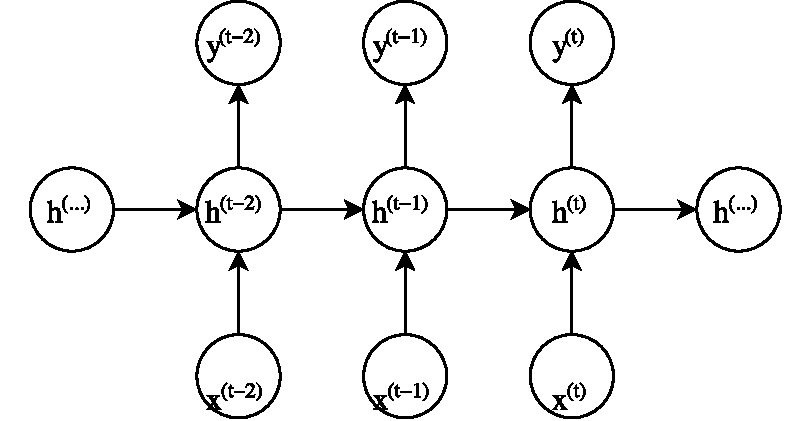
\includegraphics[width=\textwidth*2/3]{RNN.pdf}

  \caption{The ``unrolled'' computational graph for three timesteps of a recursive neural network.}
  \label{fig:rnn-computation-graph}
\end{figure}

\end{document}

%%% Local Variables:
%%% mode: latex
%%% TeX-master: t
%%% End:
